\documentclass[lettersize,journal]{IEEEtran}

\usepackage{amsmath,amsfonts,amssymb}
\usepackage{algorithm}
\usepackage{algorithmic}
\usepackage{array}
\usepackage{booktabs}
\usepackage{cite}
\usepackage{graphicx}
\usepackage{url}
\usepackage{xcolor}

\hyphenation{op-tical net-works semi-conduc-tor}

\newcommand{\ind}{\mathbb{I}}
\newcommand{\clip}{\operatorname{clip}}
\newcommand{\cvar}{\operatorname{CVaR}}

\begin{document}

\title{Constraint-Aware Hierarchical Deep Reinforcement Learning for Energy-Efficient Dynamic Edge--Cloud Workflow Scheduling}

\author{% Author information will be inserted before submission.
}

\maketitle

\begin{abstract}
Energy-aware scheduling of dynamically arriving directed-acyclic-graph (DAG)
workflows requires two coupled decisions: assigning each ready task to a
heterogeneous edge or cloud server and selecting its dynamic-voltage-and-frequency-
scaling (DVFS) ratio. A lower frequency may save dynamic power, but it also
extends execution and queue occupancy, thereby increasing the deadline risk of
the current and subsequent workflows. This paper formulates the problem as
computing-energy minimization under workflow-level deadline and reliability
requirements and proposes a constraint-aware hierarchical reinforcement learning
framework. A set of three independent dueling Double-Q estimators performs discrete
server placement by estimating energy return, deadline cost, and reliability cost.
Conditioned on the selected server, a Soft Actor--Critic controller determines
a continuous DVFS ratio. Queue-aware dense deadline credit, remaining
critical-path features, workload-level failure feedback, and workflow-level
counterfactual DVFS attribution connect delayed violations to the responsible
upper- and lower-level actions. Separate Lagrangian controllers regulate the
constraint pressure at the two levels. Evaluation uses a constraint-first
protocol: energy is compared only among methods satisfying the prescribed
empirical success probability (ESP) and reliability requirements. Across the main
four small- and medium-workflow resource configurations, the proposed method attains 90--100\% ESP at a
90\% per-run deadline-satisfaction target and 100\% reliability attainment.
Relative to the lowest-energy feasible baseline, it reduces energy by
13.45--48.93\% across the evaluated conditions.
Ablation results show that continuous DVFS provides an additional 3.31--5.13\%
energy reduction, while removing the upper deadline head collapses ESP to zero.
\end{abstract}

\begin{IEEEkeywords}
Edge--cloud computing, workflow scheduling, deep reinforcement learning,
DVFS, deadline constraint, reliability, Lagrangian optimization.
\end{IEEEkeywords}

\section{Introduction}
\label{sec:introduction}

\IEEEPARstart{E}{dge}--cloud computing combines nearby processing
resources with the computational capacity of cloud servers, enabling
applications to distribute their computation across heterogeneous
infrastructures \cite{luo2021survey}. Many applications comprise
interdependent tasks rather than isolated requests. A directed acyclic
graph (DAG) represents these dependencies: a task can execute only after
its predecessors finish and their output data become available. Scheduling
such workflows therefore requires balancing processing speed,
communication delay, and resource availability, rather than selecting
the fastest server for each task independently
\cite{topcuoglu2002,jayanetti2022}.

This problem becomes more challenging when workflows arrive dynamically.
Tasks from different workflows compete for shared servers, and a decision
that benefits the current workflow may delay another one. Dynamic
multi-workflow scheduling consequently differs from optimizing a single
DAG on an otherwise idle platform \cite{arabnejad2019}. Recent work on
interleaved workflows further demonstrates the importance of updating
task urgency according to ongoing execution and resource contention
\cite{cai2025interleaved}. For energy-aware scheduling, these interactions
also determine how much execution slack can safely be used for power
reduction.

Dynamic voltage and frequency scaling (DVFS) provides a direct means of
controlling computation energy. However, reducing frequency lowers
dynamic power while extending execution time. The frequency-independent
power consumed during this longer interval means that the lowest
frequency is not necessarily the most energy-efficient operating point
\cite{xie2017energy}. Reduced frequency can also affect transient-fault
reliability through the operating point and increased execution exposure
\cite{zhu2004,wu2018}. Thus, energy efficiency cannot be judged from
instantaneous power alone. Placement and frequency must be coordinated
with workflow deadlines and reliability requirements, as also motivated
by recent learning-based resource-management studies
\cite{oustad2025dist,esnaashari2025dream}.

Deep reinforcement learning (DRL) offers an adaptive alternative to
hand-designed scheduling rules. Existing approaches learn from workload
and resource states to improve completion time, energy consumption, or
their tradeoff \cite{chen2023,pan2024,wen2026}. Hierarchical learning is
particularly attractive because server placement is discrete whereas
frequency control is continuous \cite{zhu2026hirl}. Nevertheless,
separating these decisions into two learners does not itself resolve
their interactions. Three issues are important in the setting considered
here.

First, the effect of a scheduling action extends beyond the selected
task. A seemingly economical server may already be congested, and a
task with a short execution time may precede a long remaining critical
path. Local execution estimates must therefore be interpreted together
with workflow urgency and competing workload. Second, deadline feedback
is delayed and its causes are mixed. A workflow may already be late
because of placement or existing contention before any frequency
reduction occurs. Conversely, slowing one task can prolong a server
queue and cause another workflow to miss its deadline. Assigning an
identical terminal penalty to both learners does not distinguish these
responsibilities and can discourage useful DVFS decisions.

Third, an average deadline-satisfaction rate does not describe the
consistency of service across workload realizations. Two policies can
have similar aggregate success rates while differing substantially in
how often an individual realization meets the required target.
Accordingly, we distinguish the within-realization fraction of timely
workflows from the probability that this fraction reaches a prescribed
level. Energy reduction is meaningful only alongside the specified
deadline and reliability requirements, rather than as compensation for
violating them.

To address these issues, we propose a constraint-aware hierarchical
framework for dynamic edge--cloud workflow scheduling. The upper
controller uses three independent dueling Double-Q estimators for energy,
deadline, and reliability \cite{vanhasselt2016,wang2016dueling}; the lower
controller uses soft actor--critic (SAC) for continuous DVFS
\cite{haarnoja2018}. Both decisions incorporate remaining-path and
workload-urgency information. Their feedback is differentiated according
to the decisions each controller can influence. The main contributions
are as follows:
\begin{enumerate}
 \item We formulate active computation-energy minimization with a
 workload-level deadline success requirement and frequency-dependent
 workflow reliability. The formulation distinguishes service consistency
 from pooled deadline satisfaction.
 \item We develop queue-aware deadline credit for server placement,
 combining dense completion increments with workflow violations and
 workload-level failure feedback. Separate value estimates allow
 constraint pressure to change without redefining the energy objective.
 \item We design fixed-schedule counterfactual credit for frequency
 control, accounting for DVFS-induced lateness both within the current
 workflow and through shared queues. Separate Lagrangian controllers
 regulate the two levels according to their respective responsibilities.
\end{enumerate}
The framework is assessed through deadline-regime comparisons and
component ablations. Its feasibility is evaluated using the original
service metrics; the learning formulation does not imply a hard
real-time guarantee.

\section{Related Work}
\label{sec:related_work}

\subsection{Dynamic and Learning-Based Workflow Scheduling}

Resource scheduling in edge computing involves heterogeneous capacities,
communication costs, and changing demand \cite{luo2021survey}. For
dependent tasks, HEFT provides a foundational list-scheduling approach
based on upward ranks and earliest estimated finish times
\cite{topcuoglu2002}. Arabnejad \emph{et al.} extend the scheduling
perspective to dynamically arriving workflows with deadline and
monetary-cost requirements \cite{arabnejad2019}. Ismayilov and Topcuoglu
combine neural-network guidance with multi-objective evolutionary
optimization for dynamic workflow scheduling \cite{ismayilov2020}.
These approaches establish that placement decisions must account for
dependencies and competing workflows, not merely individual task sizes.

More recently, Cai \emph{et al.} propose urgency-based list scheduling for
deadline-constrained interleaved workflows \cite{cai2025interleaved}.
Their method uses runtime information to prioritize tasks and schedules
new arrivals together with outstanding tasks. This is directly relevant
to our use of global urgency: workflow progress changes the significance
of queue delays. Our study addresses the additional coupling introduced
by learned placement and continuous frequency control, where extending
one task's occupancy can change the urgency of other workflows.

DRL-based methods learn scheduling policies from repeated interaction.
Jayanetti \emph{et al.} optimize energy and execution time for
precedence-constrained tasks in edge--cloud environments
\cite{jayanetti2022}. Chen \emph{et al.} address collaborative scheduling
of heterogeneous workflows with execution-continuity requirements
\cite{chen2023}, while Pan and Wei introduce an online framework for
real-time cloud workflows with regularization to improve robustness
\cite{pan2024}. Wang and Sun combine DRL with ordinal optimization to
improve decision efficiency in wireless edge scheduling
\cite{wang2025ordinal}. Their emphasis on candidate-action evaluation
provides an alternative to directly exploring a large scheduling space.

Wen \emph{et al.} propose DQN-Edge, combining modified upward-rank
prioritization with context-aware attention over time and energy
feedback \cite{wen2026}. DQN-Edge already maintains separate time and
energy value estimates; value separation alone is therefore not a
distinguishing contribution of our work. Our focus is the combination
of constraint-specific costs, continuous DVFS, and differentiated
responsibility for delayed workflow outcomes. This distinction also
separates minimizing completion time from meeting a prescribed
deadline-service requirement.

\subsection{Energy- and Reliability-Aware Scheduling}

DVFS scheduling balances reduced power against longer execution.
Xie \emph{et al.} investigate energy-efficient scheduling of real-time
parallel applications on heterogeneous distributed systems
\cite{xie2017energy}. Zhu \emph{et al.} analyze the reliability impact of
energy management \cite{zhu2004}, and Zhu and Aydin study energy control
under reliability requirements \cite{zhu2006energy}. These studies
motivate frequency-dependent reliability modeling rather than treating
frequency reduction as an unrestricted energy-saving operation.

For workflow applications, Zhang \emph{et al.} consider energy and
reliability as joint scheduling objectives \cite{zhang2017}. Wu
\emph{et al.} incorporate soft-error awareness into DVFS-enabled cloud
scheduling \cite{wu2018}, and Hassan \emph{et al.} develop an energy-
and reliability-aware workflow scheduler \cite{hassan2020}. Wu
\emph{et al.} subsequently study energy-aware mapping of periodic
real-time workflows under reliability constraints, including replication
\cite{wu2023}. Recent extensions include Khaleel's integration of
asynchronous actor--critic learning with coalitional game methods
\cite{coalition2025}, and Ye \emph{et al.}'s reliability-distribution
heuristic with task clustering and processor- and task-level DVFS
\cite{ye2026}.

Reliability-aware learning has also been investigated in fog and
embedded systems. DIST coordinates distributed Q-learning with
DVFS-enabled scheduling to address energy, timing, and reliability
\cite{oustad2025dist}. DReaM jointly selects voltage--frequency settings
and fault-tolerance techniques for multicore IoT devices
\cite{esnaashari2025dream}. In the edge--cloud continuum,
Taghinezhad-Niar and Taheri propose cost-oriented scheduling under energy
and deadline constraints, with an adaptive-duplication extension for
fault tolerance \cite{taghinezhad2025recr}. These studies demonstrate
different ways of coordinating energy and reliability; their objectives
and system assumptions should not be treated as interchangeable.

Our formulation uses energy as the optimization objective and workflow
reliability as a requirement. Its scheduling emphasis is on dynamically
arriving DAGs sharing non-preemptive servers. In this setting, DVFS
changes not only the current task's execution exposure but also the
waiting time experienced by other workflows. The proposed lower-level
feedback explicitly accounts for this propagated delay.

\subsection{Hierarchical Learning and Constraint Credit}

Hierarchical learning can divide mixed discrete--continuous decisions
into conditional subproblems. The recent HiRL preprint combines
TD3-based continuous power control with DDQN-based discrete task
allocation, supported by queue-state information and deadline-oriented
prioritization \cite{zhu2026hirl}. It demonstrates the relevance of
cross-tier coordination in heterogeneous edge systems. Our hierarchy
instead selects a server before controlling its execution frequency,
and emphasizes DAG-level completion and the attribution of queue-induced
deadline losses.

Constrained reinforcement learning separates objective return from
constraint costs. Constrained policy optimization regulates policy
updates using cost constraints \cite{achiam2017}. Reward constrained
policy optimization introduces an alternative penalty signal with
multiscale updates \cite{tessler2019}, whereas PID Lagrangian control
uses constraint-error feedback to adapt penalty pressure
\cite{stooke2020}. These mechanisms inform multiplier adjustment but
do not, by themselves, determine how a delayed workflow violation
should be assigned to placement and frequency decisions. Furthermore,
an expected accumulated cost is not automatically equivalent to the
probability of meeting a workload-level service target.

Counterfactual reasoning offers a complementary approach to credit
assignment. COMA evaluates an agent's contribution using a baseline that
marginalizes its action while holding the other agents' actions fixed
\cite{foerster2018coma}. Our mechanism is different: it recomputes timing
under a fixed placement and server order while restoring selected
execution frequencies. The resulting comparison estimates the
additional lateness associated with DVFS under that schedule; it is
not a globally reoptimized alternative schedule. Combining this
responsibility signal with queue-aware placement credit and
workload-level deadline feedback is the central focus of our method.

\section{System Model and Problem Formulation}
\label{sec:model}

\subsection{Workflow and Heterogeneous Resources Model}

The principal notation is summarized in Table~\ref{tab:notation}.
Let $\mathcal W$ denote the workflows in one workload realization.
A workflow $w$ is modeled as a DAG with task set
$\mathcal{N}=\{1,2,\ldots,n\}$ and precedence edge set
$\mathcal{E}$. It is characterized by arrival time $a_w$,
relative deadline $D_w>0$, and reliability requirement $R_w\in(0,1)$:
\begin{equation}
    w=\{\mathcal{N},\mathcal{E},a_w,D_w,R_w\}.
\end{equation}
An edge $(i,j)\in\mathcal{E}$ indicates that task $j$ can
start only after task $i$ finishes and its output data
have arrived at the assigned server.
For task $i\in\mathcal{N}$, $\Phi_{\mathrm{pred}}(i)$ and
$\Phi_{\mathrm{succ}}(i)$ denote its immediate predecessor
and successor sets, respectively.
Task indices are local to each workflow; the workflow index
is omitted when the context is clear.

\begin{table}[t]
\centering
\caption{Principal notation.}
\label{tab:notation}
\renewcommand{\arraystretch}{1.08}
\begin{tabular}{@{}p{0.29\columnwidth}p{0.64\columnwidth}@{}}
\toprule
Symbol & Definition \\
\midrule
$\mathcal{N},\mathcal{E}$ & Task and precedence-edge sets \\
$a_w,D_w,R_w$ & Arrival time, relative deadline, and reliability requirement \\
$L_i,D_{ij}$ & Task workload and inter-task data volume \\
$\mathcal{M},m_i$ & Server set and assigned server of task $i$ \\
$F_m,B_{mm'}$ & Maximum frequency and link bandwidth \\
$f_i,\rho_i$ & Execution frequency and frequency scaling ratio \\
$ET_i,WT(i)$ & Execution duration and waiting duration \\
$RT(i),ST(i),FT(i)$ & Data-ready, start, and finish times \\
$P_i,E_i$ & Active power and computation energy of task $i$ \\
$T_w,E_w,\mathcal{R}_w$ & Workflow response time, computation energy, and reliability \\
$\mathrm{SR},\Gamma,\eta$ & Within-run success rate, rate target, and probability target \\
$\mathrm{ESP}_{\Gamma}$ & Empirical probability of meeting the rate target \\
$\lambda_m(f),\mu_D^H,\mu_D^L$ & Fault rate and upper/lower deadline multipliers \\
\bottomrule
\end{tabular}
\end{table}

Let $\mathcal{M}=\mathcal{M}^{\mathrm{e}}\cup
\mathcal{M}^{\mathrm{c}}$ denote the server set, where
$\mathcal{M}^{\mathrm{e}}$ and $\mathcal{M}^{\mathrm{c}}$
represent edge and cloud servers, respectively.
Edge servers offer low communication latency but limited
computational capacity, whereas cloud servers provide
greater computational capacity with longer transmission
delays. Each server executes at most one task at a time,
and task execution is non-preemptive.
Server $m\in\mathcal{M}$ has a maximum operating frequency
$F_m$.


\subsection{Task Execution and Communication Model}

For task $i\in\mathcal{N}$, let $L_i$ denote its computational
workload in processor cycles, $m_i\in\mathcal{M}$ its assigned
server, and $f_i$ its execution frequency.
Its execution time is
\begin{equation}
    ET_i=\frac{L_i}{f_i}.
    \label{eq:execution_time}
\end{equation}

For each edge $(i,j)\in\mathcal{E}$, let $D_{ij}$ denote
the transmitted data volume in bits.
Let $B_{mm'}$ denote the bandwidth in bits per second
between servers $m$ and $m'$. Bandwidths are treated as effective,
fixed transfer rates.
The communication delay is
\begin{equation}
    c_{ij}=
    \begin{cases}
        \dfrac{D_{ij}}{B_{m_i m_j}}, & m_i\neq m_j,\\[2mm]
        0, & m_i=m_j.
    \end{cases}
    \label{eq:communication_delay}
\end{equation}

Let $RT(i)$, $ST(i)$, and $FT(i)$ denote the data-ready,
start, and finish times of task $i$, respectively.
Task $i$ becomes data-ready when all required predecessor
outputs have arrived:
\begin{equation}
    RT(i)=
    \begin{cases}
        a_w, & \Phi_{\mathrm{pred}}(i)=\varnothing,\\[2mm]
        \displaystyle
        \max_{j\in\Phi_{\mathrm{pred}}(i)}
        \{FT(j)+c_{ji}\}, & \text{otherwise}.
    \end{cases}
    \label{eq:ready_time}
\end{equation}

After its input data have arrived, task $i$ may still wait
before execution. Let $WT(i)$ denote this waiting time,
including scheduling and server-queue delays.
Waiting is determined by the dispatch rule and server queue; it is
not an independent scheduling control. Execution intervals of tasks
assigned to the same server do not overlap.
The start and finish times are
\begin{align}
    ST(i)&=RT(i)+WT(i), \label{eq:start_time}\\
    FT(i)&=ST(i)+ET_i. \label{eq:finish_time}
\end{align}

Workflow $w$ completes when all its tasks have finished.
Its response time, measured from arrival to completion, is
\begin{equation}
    T_w=\max_{i\in\mathcal{N}}FT(i)-a_w.
    \label{eq:workflow_makespan}
\end{equation}


\subsection{Power Model and Energy Model}
\label{subsec:energy_model}

DVFS adjusts the execution frequency of task $i$ through the ratio
$\rho_i$. For its assigned server $m_i$, the execution frequency is
\begin{equation}
 f_i=\rho_iF_{m_i},\qquad \underline\rho_{m_i}\leq\rho_i\leq1,
 \label{eq:task_frequency}
\end{equation}
where $F_m$ and $\underline\rho_m$ are the maximum frequency and minimum
supported frequency ratio of server $m$, respectively; the minimum
frequency is $F_m^{\min}=\underline\rho_m F_m$.
Following the frequency-dependent power models
in~\cite{xie2017energy,zhu2006energy}, we adopt a cubic active-power model:
\begin{equation}
 P_i=P_{m_i}^{\mathrm{ind}}+P_{m_i}^{\mathrm{dyn}}\rho_i^3,
 \label{eq:task_power}
\end{equation}
where $P_m^{\mathrm{ind}}\geq0$ is frequency-independent active power and
$P_m^{\mathrm{dyn}}>0$ is dynamic power at the maximum frequency.
The frequency remains constant during task execution. With execution
time $ET_i=L_i/f_i$, the task's computation energy is
\begin{equation}
 E_i=P_iET_i
 =\frac{L_i}{F_{m_i}}\left(
 \frac{P_{m_i}^{\mathrm{ind}}}{\rho_i}
 +P_{m_i}^{\mathrm{dyn}}\rho_i^2\right).
 \label{eq:task_energy}
\end{equation}

Reducing frequency lowers dynamic power but prolongs execution and
therefore increases the frequency-independent energy component.
Minimizing $E_i$ with respect to $\rho_i$ over the supported interval gives
the energy-efficient operating ratio of server $m$:
\begin{equation}
 \rho_m^{\mathrm{ee}}=\min\!\left\{1,\max\!\left\{
 \underline\rho_m,
 \left(\frac{P_m^{\mathrm{ind}}}{2P_m^{\mathrm{dyn}}}\right)^{1/3}
 \right\}\right\}.
 \label{eq:rhoee}
\end{equation}
This ratio depends on server power characteristics, not task workload;
meeting timing and reliability requirements may require a higher
execution frequency.
The total computation energy of workflow $w$ is
\begin{equation}
 E_w=\sum_{i\in\mathcal N}E_i.
 \label{eq:workflow_energy}
\end{equation}
Only active computation energy is considered; idle and communication
energy are excluded.


\subsection{Deadline and Reliability Constraints}

A workflow meets its deadline when its response time satisfies
\begin{equation}
 T_w\leq D_w.
 \label{eq:deadline_constraint}
\end{equation}
The response time includes communication, waiting, and execution.
The service-level condition below specifies the required fraction
of workflows meeting this inequality.

Following the transient-fault model in~\cite{zhu2004},
fault occurrences during task execution are assumed to
follow a Poisson process. We adopt the DVFS-dependent
fault-rate model used in~\cite{wu2018}.
Let $\lambda_m^{\max}$ denote the fault rate of server $m$
at its maximum frequency $F_m$, $F_m^{\min}$ its minimum
operating frequency, and $\kappa_m>0$ its sensitivity
to frequency scaling. For task $i$ executed on server $m_i$
at frequency $f_i$, the fault rate is
\begin{equation}
    \lambda_{m_i}(f_i)=\lambda_{m_i}^{\max}
    10^{\kappa_{m_i}
    \frac{F_{m_i}-f_i}{F_{m_i}-F_{m_i}^{\min}}}.
    \label{eq:dvfs_fault_rate}
\end{equation}

Without task replication or recovery, the reliability
of task $i$ is the probability of fault-free execution:
\begin{equation}
    \mathcal{R}_i
    =e^{-\lambda_{m_i}(f_i)ET_i}.
    \label{eq:task_reliability}
\end{equation}
Assuming independent task failures, workflow reliability is
\begin{equation}
    \mathcal{R}_w=\prod_{i\in\mathcal{N}}\mathcal{R}_i.
    \label{eq:workflow_reliability}
\end{equation}
The reliability constraint is
\begin{equation}
    \mathcal{R}_w\geq R_w.
    \label{eq:reliability_constraint}
\end{equation}


\subsection{Service-Level Requirement and Optimization Objective}
\label{subsec:objective}

For a workload realization $\mathcal W$, define the deadline success
rate as
\begin{equation}
 \mathrm{SR}=\frac{1}{|\mathcal W|}
 \sum_{w\in\mathcal W}\ind(T_w\leq D_w),
 \label{eq:success_rate}
\end{equation}
where $\ind(\cdot)$ is the indicator function. Let $\Gamma\in(0,1]$
be the required success rate within a realization, and
$\eta\in(0,1]$ the required probability of achieving it.
The service-level deadline constraint is
$\Pr_\pi(\mathrm{SR}\geq\Gamma)\geq\eta$, where the probability is
over workload realizations and any policy randomization.

Let $\pi$ denote an online scheduling policy that selects $m_i$ and
$\rho_i$ from currently available information. The objective is
\begin{align}
 \min_{\pi}\quad&
 \mathbb E_\pi\!\left[\sum_{w\in\mathcal W}E_w\right]
 \label{eq:objective}\\
 \text{s.t.}\quad&
 \Pr_\pi(\mathrm{SR}\geq\Gamma)\geq\eta,\nonumber\\
 &\mathcal R_w\geq R_w,\qquad w\in\mathcal W,\nonumber\\
 &m_i\in\mathcal M,\quad
 \underline\rho_{m_i}\leq\rho_i\leq1,\nonumber
\end{align}
together with the precedence, communication, and non-preemptive
server-capacity conditions above. Energy is the sole minimized
quantity; deadlines and reliability define feasibility.
For a fixed number of workflows per realization, minimizing total
energy and minimizing mean energy per workflow differ only by a
constant factor.

On $N_{\mathrm{test}}$ independent test realizations, the empirical
success probability is
\begin{equation}
 \mathrm{ESP}_{\Gamma}=
 \frac{1}{N_{\mathrm{test}}}
 \sum_{e=1}^{N_{\mathrm{test}}}\ind(\mathrm{SR}_e\geq\Gamma).
 \label{eq:esp}
\end{equation}
Here $\mathrm{SR}_e$ is \eqref{eq:success_rate} evaluated on realization
$e$, whose workflow set is denoted by $\mathcal W_e$.
Thus, $\Gamma=0.90$ requires at least 90\% of workflows in a realization
to finish on time; $\mathrm{ESP}_{0.90}$ measures how often this
requirement is met across test realizations. It estimates the
service probability and is distinct from the mean of
$\mathrm{SR}_e$. Likewise, reliability attainment records whether
$\mathcal R_w\geq R_w$; 100\% attainment does not mean
$\mathcal R_w=1$.

\section{Proposed Method}
\label{sec:method}

\subsection{Decision Process and Hierarchical Framework}
\label{subsec:framework}

Server placement and frequency control are coordinated through a
hierarchical partially observable decision process. The two learners
observe task and resource features rather than the complete scheduling
state. We describe the process by
\begin{equation}
 \mathfrak P=\langle\mathcal K,\mathcal S,\mathcal A,\mathcal P,
 \Omega,\mathcal O,\mathbf r,\boldsymbol\delta\rangle,
 \label{eq:method_pomdp}
\end{equation}
where:
\begin{itemize}
 \item $\mathcal K=\{H,L\}$ is the set of upper and lower learners.
 \item $\mathcal S$ is the global state space, including workflow progress,
 server queues, current time, and the arrival-process state.
 \item $\mathcal A$ is the joint action space. For a ready task $i$,
 $a_t=(m_i,\rho_i)$ specifies its server and frequency ratio, with
 $\mathcal A=\bigcup_{m\in\mathcal M}
 (\{m\}\times[\underline\rho_m,1])$.
 \item $\mathcal P(s'\mid s,a)$ is the state-transition kernel induced by
 task execution, queue evolution, and workflow arrivals.
 \item $\Omega=\Omega_H\times\Omega_L$ is the joint observation space,
 where $\Omega_H$ and $\Omega_L$ contain the feature representations
 $s_t^H$ and $s_t^L$, respectively.
 \item $\mathcal O$ is the observation kernel. Upper observations are
 obtained from the current state; lower observations additionally depend
 on the server selected by the upper learner. The encoders used here
 are deterministic.
 \item $\mathbf r=(r_{E,t}^H,r_t^L)$ contains the upper energy reward and
 lower frequency-control reward. Deadline and reliability costs are
 specified separately in the following subsections.
 \item $\boldsymbol\delta=(\delta_E,\delta_D,\delta_R,\delta_L)$ contains
 the discount factors for upper energy and constraint estimation and
 lower actor--critic learning, each taking a value in $(0,1]$.
\end{itemize}

The index $t$ denotes a task-dispatch decision, not a fixed physical-time
interval. A common ready-task ordering rule supplies task $i$ of workflow
$w$; task ordering is not learned. The upper learner first selects $m_i$
from $s_t^H$, after which the lower learner determines $\rho_i$ from the
selected-server observation $s_t^L$. Each trajectory covers the complete
execution of a workload.

Placement determines communication and contention, whereas frequency
control determines execution time and active energy on the selected
server. We therefore factorize the policy into a discrete upper policy
and a conditional continuous lower policy:
\begin{equation}
 \pi(m_i,\rho_i\mid s_t)
 =\pi_H(m_i\mid s_t^H)\,
   \pi_L(\rho_i\mid s_t^L,m_i),
 \label{eq:method_factorization}
\end{equation}
where $s_t^H$ and $s_t^L$ are the respective feature-based observations.
They summarize, rather than fully reconstruct, the Markov state.
The upper learner uses three D3QN estimators for energy, deadline, and
reliability, while the lower learner uses soft actor--critic (SAC) for
DVFS. Both learn from the same trajectories: the upper action is evaluated
after the lower frequency decision, and both observe global deadline
pressure. Their constraint costs distinguish placement consequences from
the additional losses caused by frequency reduction.

For the current workflow $w$, retain the local task notation
$\mathcal N$ and $n=|\mathcal N|$ from the system model. Let
$\mathcal I_w$ contain its decision indices and $[x]_+=\max(0,x)$.
In sums over decisions from different workflows, $n$ and $D_w$ refer
to the workflow of the corresponding decision.
We use $\mu$, rather than $\lambda$, for constraint multipliers to
distinguish them from the transient-fault rates in the system model.
The actual energy remains $E_i$; $\widehat E(i,m,\rho)$ denotes the same
energy model evaluated for a candidate server and frequency. The
energy-efficient ratio $\rho_m^{\mathrm{ee}}$ is defined in the power and
energy model.

\subsection{Upper-Level Server Selection}
\label{subsec:high}

\subsubsection{State Representation}

The upper state contains task workload and deadline slack, together with
server-specific estimates of communication time, execution time, queue
waiting, full-frequency energy, and task failure probability. Server
occupancy and recent assignment history describe resource contention.
Current slack alone does not account for unfinished successors. Let
$\ell_i$ be an estimate of the completion time still required after task
$i$, obtained from its upward rank after removing its mean execution
time. For candidate
server $m$, let $\widehat{ST}(i,m)$ and $\widehat{FT}(i,m)$ be its
estimated start and full-frequency finish times under the current queues.
Its predicted workflow response time is
\begin{equation}
 \widehat T(i,m)=\widehat{FT}(i,m)-a_w+\ell_i.
 \label{eq:method_predicted_finish}
\end{equation}
With a small margin $\zeta$, the available execution budget is
$b(i,m)=(1-\zeta)[a_w+D_w-\widehat{ST}(i,m)-\ell_i]$.
Let $\widehat{ET}(i,m)=L_i/F_m$ denote full-frequency execution time on candidate
server $m$. The state includes this budget and the indicative frequency
\begin{equation}
 \widehat\rho(i,m)=
 \begin{cases}
 \min\{1,\max\{\rho_m^{\mathrm{ee}},\widehat{ET}(i,m)/b(i,m)\}\},&b(i,m)>0,\\
 1,&b(i,m)\leq0,
 \end{cases}
 \label{eq:method_time_frequency}
\end{equation}
This frequency is a state feature, not a hard deadline-feasibility
guarantee.

To expose congestion beyond the current workflow, let $\mathcal W_t$
contain all released, unfinished workflows and let $h_w$ estimate their
remaining critical-path duration, accounting for the residual execution
of running tasks. At current physical time $t_{\mathrm{now}}$, and with
$\epsilon>0$ to prevent division by zero, define
\begin{align}
 p_w&=\frac{h_w}{\max\{a_w+D_w-t_{\mathrm{now}},\epsilon\}},\nonumber\\
 \chi_t&=\tanh\!\left(\frac{\sum_{w\in\mathcal W_t}p_w}{|\mathcal M|}\right),\quad
 \chi_t^{\max}=\frac{\min\{2,\max_{w\in\mathcal W_t}p_w\}}{2},
 \label{eq:method_global_pressure}
\end{align}
Both features are zero when $\mathcal W_t$ is empty. They enter both levels,
allowing placement and frequency control to observe shared deadline
pressure rather than only local slack. Time features are normalized by
the corresponding workflow deadline.

\subsubsection{Action Selection}

The upper learner maintains independent energy-return, deadline-cost,
and reliability-cost estimators, denoted by $Q_E$, $Q_D$, and $Q_R$.
Each uses the dueling representation~\cite{wang2016dueling}
\begin{equation}
 Q_h(s,m)=V_h(s)+A_h(s,m)
 -\frac{1}{|\mathcal M|}\sum_{m'\in\mathcal M}A_h(s,m'),
 \quad h\in\{E,D,R\}.
 \label{eq:method_dueling}
\end{equation}
The estimators have separate parameters; their outputs are combined
only for action selection. Given multipliers $\mu_D^H$ and $\mu_R^H$,
the exploitation action is
\begin{equation}
 m_i=\arg\max_{m\in\mathcal M}
 \left\{Q_E(s_t^H,m)-\mu_D^H[Q_D(s_t^H,m)]_+
 -\mu_R^H Q_R(s_t^H,m)\right\}.
 \label{eq:method_high_action}
\end{equation}
The nonnegative deadline projection prevents a negative cost estimate
from being treated as a scheduling benefit. Training uses
$\varepsilon$-greedy exploration over the available servers.

\subsubsection{Reward and Constraint Costs}

\paragraph{Energy.}
Let $\bar E_i=\operatorname{median}_{m\in\mathcal M}
\widehat E(i,m,1)$ be its full-frequency reference scale. The energy feedback is
\begin{equation}
 r_{E,t}^H=\frac{\bar E_i-E_i}{n\bar E_i}.
 \label{eq:method_high_energy}
\end{equation}
This dimensionless surrogate exposes the realized energy difference
while limiting the dependence of reward magnitude on workflow size.

\paragraph{Deadline.}
Let $\Delta T_{w,t}$ be the nonnegative increment in the predicted
partial workflow response time after decision $t$. Terminal feedback
reconciles these increments with the completed response time, such that
$\sum_{t\in\mathcal I_w}\Delta T_{w,t}=T_w$.
Let $q_t$ be the selected task's waiting time caused by server contention,
excluding prerequisite communication and waiting before dispatch.
It is the server-contention component of $WT(i)$, not the
communication delay $c_{ji}$ or the execution duration $ET_i$.
The dense cost is
\begin{equation}
 d_t=\frac{\Delta T_{w,t}}{D_w}
 +\beta_q\frac{q_t}{nD_w}.
 \label{eq:method_dense_cost}
\end{equation}
The queue term provides credit to tasks whose waiting does not increase
the current workflow completion frontier. It also participates in
distributing the final miss cost. Define
$b_w=\mathbb{I}(T_w>D_w)$ and
$\omega_t=d_t/\sum_{j\in\mathcal I_w}d_j$.
For a completed trajectory $e$ with workflow set $\mathcal W_e$, let
$\mathrm{SR}_e$ be its deadline success rate as defined in the problem
formulation. The service-level failure indicator is
$z_e=\mathbb{I}(\mathrm{SR}_e<\Gamma)$.
To allocate this trajectory-level failure, define the avoidable
predicted completion regret
$\Delta_t^{\mathrm{sel}}=[\widehat T(i,m_i)-\min_m\widehat T(i,m)]_+/D_w$
and normalize it
over all decision indices $\mathcal I_e$ of the run as
$\nu_t=\Delta_t^{\mathrm{sel}}/\sum_{j\in\mathcal I_e}\Delta_j^{\mathrm{sel}}$.
With failure-credit coefficient $\beta_{\mathrm{miss}}$, the final deadline cost is
\begin{equation}
 g_{D,t}^H=d_t+\beta_{\mathrm{miss}} b_w\omega_t
 +\beta_{\mathrm{miss}} z_e\nu_t,
 \label{eq:method_high_deadline}
\end{equation}
The same coefficient controls both failure-credit terms. Zero denominators
are handled by uniform allocation over the corresponding indices.
Thus, ESP failure credit supplements, rather than replaces, the dense
signal. For queue calibration, let $\mathcal I_{\mathrm{cal}}$ contain
the decision indices in an initial observation window and let
$\theta_q\in(0,1)$ be the desired queue share of the dense cost. Set
\begin{equation}
 \beta_q=\frac{\theta_q}{1-\theta_q}
 \frac{\sum_{t\in\mathcal I_{\mathrm{cal}}}\Delta T_{w,t}/D_w}
 {\sum_{t\in\mathcal I_{\mathrm{cal}}}q_t/(nD_w)}.
 \label{eq:method_queue_calibration}
\end{equation}
The coefficient is then held fixed;
it is zero when no queue waiting is observed.

\paragraph{Reliability.}
The completed workflow reliability deficit is
$\ell_w^R=[\ln R_w-\ln\mathcal R_w]_+$.
The reliability cost $g_{R,t}^H$ equals $\ell_w^R$ at the last decision
of workflow $w$ and zero at its other decisions. Delayed feedback is
attached to the corresponding transition after completion.

\subsubsection{Value Update}

The three estimators use Double-Q targets~\cite{vanhasselt2016} with a
common next server selected by the online score in
\eqref{eq:method_high_action}. Let this server be $m^*$, let bars denote
target estimators, let $\delta_h$ be discount factors, and let $\iota_t$
indicate the end of the complete scheduling trajectory. Then
\begin{align}
 y_{E,t}&=r_{E,t}^H+\delta_E(1-\iota_t)\bar Q_E(s_{t+1}^H,m^*),\nonumber\\
 y_{D,t}&=g_{D,t}^H+\delta_D(1-\iota_t)[\bar Q_D(s_{t+1}^H,m^*)]_+,\nonumber\\
 y_{R,t}&=g_{R,t}^H+\delta_R(1-\iota_t)\bar Q_R(s_{t+1}^H,m^*).
 \label{eq:method_high_targets}
\end{align}
For replay minibatch $\mathcal B$, each estimator minimizes
\begin{equation}
 \mathcal L_h=\mathbb E_{\mathcal B}\left[
 \operatorname{Huber}\!\left(Q_h(s_t^H,m_i)-y_{h,t}\right)\right],
 \quad h\in\{E,D,R\}.
 \label{eq:method_high_loss}
\end{equation}
Transitions retain the
global chronological order, including switches between workflows,
because their queues and future costs are coupled.

\subsection{Lower-Level Frequency Control}
\label{subsec:low}

\subsubsection{State and Action}

The lower observation $s_t^L$ contains the selected task's workload,
full-frequency execution time, predicted waiting time, remaining
deadline, server power characteristics, and reliability requirement.
It also includes $\chi_t$ and $\chi_t^{\max}$, so that frequency control
can respond to urgency outside the current workflow.
The learner uses SAC~\cite{haarnoja2018}, with a stochastic actor
and two soft critics. The actor produces a squashed-Gaussian
frequency proposal $\rho_i^a\in[\rho_0,1]$, where $\rho_0$ is the
common minimum proposal ratio. The executed ratio is
\begin{equation}
 \rho_i=\max\{\rho_i^a,\rho_{m_i}^{\mathrm{ee}}\}.
 \label{eq:method_frequency_floor}
\end{equation}
The floor excludes frequencies below the energy-efficient operating point; it
does not enforce the time-based frequency in
\eqref{eq:method_time_frequency}.

\subsubsection{Reward and Responsibility Credit}

\paragraph{Energy and local delay.}
For the selected server and the same pre-decision queue, compare the
executed action with full-frequency execution. Define
$\Delta E_i=\widehat E(i,m_i,1)-E_i$ and
$\Delta ET_i=[ET_i-L_i/F_{m_i}]_+$.
If $T_{w,t}^{\mathrm{pre}}$ is the partial workflow response time before
the decision, the local delay shaping cost is
\begin{equation}
 h_t=\frac{\Delta ET_i}{\max\{D_w-T_{w,t}^{\mathrm{pre}},\zeta D_w\}}.
 \label{eq:method_local_delay}
\end{equation}
Let $\mathcal Z_E$ and $\mathcal Z_h$ denote separate standardization
of energy saving and delay using replay-minibatch means and standard
deviations, with positive scale floors and bounded normalized values.

\paragraph{Deadline responsibility.}
A local timing comparison cannot account for delays passed to later
tasks on the same server. We therefore evaluate completed trajectories
under fixed placement, server execution order, communication delays,
and decision-release times. Restoring execution to full frequency
propagates through both workflow-precedence and server-order edges.
This replay changes execution durations, not the scheduling decisions.

Let $T_v^{\mathrm{all}}$ be workflow $v$'s response time when all tasks are
restored to full frequency, and $T_v^{u\to1}$ its response time when only
workflow $u$ is restored. With normalized lateness
$\mathcal L(T,D)=[(T-D)/D]_+$, define
\begin{align}
 d_v^L&=\min\{1,[\mathcal L(T_v,D_v)-\mathcal L(T_v^{\mathrm{all}},D_v)]_+\},\nonumber\\
 M_{uv}&=[\mathcal L(T_v,D_v)-\mathcal L(T_v^{u\to1},D_v)]_+.
 \label{eq:method_counterfactual_marginal}
\end{align}
The first quantity measures the victim's DVFS-attributable lateness;
the second measures the contribution associated with source workflow
$u$. Allocate each victim's cost back to its sources as
\begin{equation}
 G_u=\sum_{v\in\mathcal W_e}
 \frac{M_{uv}}{\sum_{u'\in\mathcal W_e}M_{u'v}}\,d_v^L.
 \label{eq:method_source_credit}
\end{equation}
If every marginal for a victim is zero, its cost is allocated in
proportion to the sources' total execution slowdown. With positive
attributable slowdown, $\sum_uG_u=\sum_vd_v^L$, avoiding repeated
charging of the same victim cost. Source credit is distributed among
its frequency actions by
\begin{equation}
 g_{D,t}^L=G_w\frac{\Delta ET_i}
 {\sum_{j\in\mathcal N}\Delta ET_j},\qquad t\in\mathcal I_w,
 \label{eq:method_low_deadline_credit}
\end{equation}
using uniform allocation if the denominator is zero. This conditional
responsibility measure includes queue delays imposed on other
workflows; it is not a reoptimized counterfactual schedule.

\paragraph{Reliability responsibility.}
Let $\widehat{\mathcal R}_{w,t}(f)$ be projected workflow reliability
when the current task executes at frequency $f$, with previous decisions and the
remaining-task estimate held fixed. Define
\begin{align}
 u_{R,t}(f)&=
 \frac{[\ln R_w-\ln\widehat{\mathcal R}_{w,t}(f)]_+}{-\ln R_w},\nonumber\\
 g_{R,t}^L&=[u_{R,t}(f_i)-u_{R,t}(F_{m_i})]_+,
 \label{eq:method_low_reliability}
\end{align}
for $0<R_w<1$. The lower controller is thus charged for the additional
projected deficit caused by its frequency choice, not the deficit
already present at full frequency. Its replay reward is
\begin{equation}
 r_t^L=\mathcal Z_E(\Delta E_i)-\mathcal Z_h(h_t)
 -\mu_D^L g_{D,t}^L-\mu_R^L g_{R,t}^L.
 \label{eq:method_low_reward}
\end{equation}
The local delay term provides shaping, while the two multipliers
regulate responsibility-based constraint costs.

\subsubsection{Actor--Critic Update}

Let $Q_1^L,Q_2^L$ be the critics, $\psi$ the actor parameters,
$\alpha$ the entropy coefficient, and $\delta_L$ the discount factor.
For a sampled next proposal $\rho'{}^a\sim\pi_\psi(\cdot\mid s_{t+1}^L)$,
the soft TD target is
\begin{align}
 y_t^L=r_t^L+\delta_L(1-\iota_t)\big[&\min_{j=1,2}
 \bar Q_j^L(s_{t+1}^L,\rho'{}^a)\nonumber\\
 &-\alpha\ln\pi_\psi(\rho'{}^a\mid s_{t+1}^L)\big].
 \label{eq:method_sac_target}
\end{align}
The critics minimize the squared TD error at the stored executed
action $\rho_i$. The actor minimizes
\begin{equation}
 \mathcal L_\pi=\mathbb E\!\left[
 \alpha\ln\pi_\psi(\rho^a\mid s^L)
 -\min_{j=1,2}Q_j^L(s^L,\rho^a)\right].
 \label{eq:method_sac_actor}
\end{equation}
Here the policy density refers to the proposal before the operating
floor in \eqref{eq:method_frequency_floor} is applied.

\subsection{Joint Learning and Constraint Adaptation}
\label{subsec:joint}

Both policies interact with the same environment before their updates.
After a complete scheduling trajectory, workflow outcomes determine
the upper failure credits and lower counterfactual credits. These are
attached to chronological transitions and stored in the respective
replay buffers. The upper estimators and the lower actor--critic are
then updated from replay, and their target networks are softly updated.
No additional coordination network is introduced.

Deadline multipliers use proportional--integral constraint feedback,
following the control perspective of Lagrangian
methods~\cite{stooke2020}. Let $\mathcal B_H$ and $\mathcal B_L$ be recent
trajectory windows, and $\vartheta\in(0,1]$ the fraction of the upper
tail used for lower feedback. The two statistics are, respectively,
\begin{equation}
 J_H=\frac{1}{|\mathcal B_H|}\sum_{e\in\mathcal B_H}z_e,
 \qquad
 J_L=\operatorname{CVaR}^{\mathrm{upper}}_{\vartheta}
 \left(\left\{\frac{\sum_{v\in\mathcal W_e}d_v^L}{|\mathcal W_e|}
 \right\}_{e\in\mathcal B_L}\right),
 \label{eq:method_dual_statistics}
\end{equation}
where the empirical upper-tail CVaR is the mean of the largest
$\lceil\vartheta|\mathcal B_L|\rceil$ values. Thus, upper feedback observes
the failure probability underlying ESP, whereas lower feedback
observes the tail of DVFS-attributable lateness, not total system
failure. For level $j\in\{H,L\}$, let $b_j$ be its budget, $\tau_j$
the integral step size, $k_j$ the proportional gain, $I_j$ the integral
state, and $\mu_{D,\max}^j$ the multiplier bound. With
$e_j=J_j-b_j$, update
\begin{align}
 I_j&\leftarrow\Pi_{[0,\mu_{D,\max}^j]}(I_j+\tau_j e_j),\nonumber\\
 \mu_D^j&\leftarrow\Pi_{[0,\mu_{D,\max}^j]}(I_j+k_j e_j).
 \label{eq:method_pi_dual}
\end{align}
Here $\Pi$ denotes interval projection. The upper budget $b_H$ controls the tolerated service-failure
frequency; $b_H=1-\eta$ aligns it with the deadline probability target
in \eqref{eq:objective}. The lower budget $b_L$ controls attributable
lateness and is not another definition of ESP.

Reliability adaptation uses completed workflow outcomes. Let
$\tau_R^H,\tau_R^L$ be reliability update step sizes and
$\mu_{R,\max}^H,\mu_{R,\max}^L$ their multiplier bounds. The upper
multiplier accumulates the log-reliability deficit after each completed
workflow, while the lower multiplier compares the recent binary
violation frequency $\bar b_R$ with a small budget $b_R$:
\begin{align}
 \mu_R^H&\leftarrow
 \Pi_{[0,\mu_{R,\max}^H]}(\mu_R^H+\tau_R^H\ell_w^R),\nonumber\\
 \mu_R^L&\leftarrow
 \Pi_{[0,\mu_{R,\max}^L]}(\mu_R^L+\tau_R^L(\bar b_R-b_R)),
 \label{eq:method_reliability_duals}
\end{align}
where $\bar b_R$ averages $\mathbb{I}(\mathcal R_w<R_w)$ over recent
completed workflows. These updates are intentionally asymmetric: upper reliability
pressure is nondecreasing, whereas lower pressure decreases when its
violation budget is satisfied.

Placement thus learns from end-to-end outcomes, while frequency control
learns from the additional losses attributed to slowdown. The normalized
feedback provides learning surrogates for the physical objective;
service-level feasibility is assessed using the original deadline and
reliability criteria, rather than inferred from the shaped return.


\section{Experimental Evaluation}
\label{sec:experiments}

The experiments examine three questions: whether the proposed hierarchy
reduces computation energy while meeting the service requirements;
whether its policy remains effective when the deadline distribution
changes; and which components account for the observed behavior.
Energy, deadline service attainment, and reliability attainment are
reported separately to distinguish valid energy savings from reductions
obtained by violating constraints.

\subsection{Experimental Setup}
\label{subsec:experiment_setup}

\subsubsection{Workflows and Resource Configurations}

The simulator uses DAG topologies from five scientific workflow families:
CyberShake, Epigenomics, Inspiral, Montage, and SIPHT. The Small pool
contains five templates with 24--30 tasks. The Medium pool contains these
five templates and five larger templates, giving 24--58 tasks per
workflow. Thus, Medium is a cumulative template pool rather than a
collection consisting exclusively of larger DAGs. A template is sampled
uniformly for each workflow. Task workloads and edge data volumes are
sampled uniformly from $[0.5,20]\times10^9$ cycles and $[1,30]$ MB,
respectively. The topologies are benchmark-derived, whereas these
execution and communication parameters are synthetic.

Each workload realization contains 20 dynamically arriving workflows.
Interarrival times are exponentially distributed with rate
$0.1\ \mathrm{s}^{-1}$, corresponding to a mean interval of 10 s.
Table~\ref{tab:experiment_scenarios} defines a two-by-two design involving
workload size and relative resource provision. Expanding S26 to S37
increases the server count from 26 to 37; expanding M37 to M53 increases
it from 37 to 53. These changes apply similar expansion factors to both
workload scales while approximately preserving the edge--cloud ratio.
All policies are trained for their own workload--resource configuration;
a checkpoint with a different number of server outputs is not used as
the trained model of another configuration.

\begin{table}[t]
\centering
\caption{Workload--resource configurations. Mean task counts are averages
over the template pools, not measurements of system utilization.}
\label{tab:experiment_scenarios}
\footnotesize
\setlength{\tabcolsep}{4pt}
\renewcommand{\arraystretch}{1.08}
\begin{tabular}{@{}llrrrr@{}}
\toprule
ID & Pool & Tasks & Mean & Edge & Cloud \\
\midrule
S26 & Small & 24--30 & 27.6 & 20 & 6 \\
S37 & Small & 24--30 & 27.6 & 28 & 9 \\
M37 & Medium & 24--58 & 39.3 & 28 & 9 \\
M53 & Medium & 24--58 & 39.3 & 40 & 13 \\
\bottomrule
\end{tabular}
\end{table}

The common resource model contains three edge profiles and two cloud
profiles, listed in Table~\ref{tab:experiment_resources}. Edge profiles
are allocated approximately equally; the two cloud profiles are also
allocated approximately equally. Frequencies and the two power
components are independently perturbed by up to $\pm5\%$ around their
nominal values. Resource generation uses seed 42, so every method in a
configuration observes the same server pool. Edge--edge, edge--cloud,
and cloud--cloud links have bandwidths of 1, 0.1, and 10 Gbit/s,
respectively. The shared simulator orders dispatchable tasks by
increasing workload. Each server executes one task at a time without
preemption, as specified in Section~\ref{sec:model}.

\begin{table}[t]
\centering
\caption{Nominal server profiles. Power components follow
\eqref{eq:task_energy}; fault rates are measured at maximum frequency.}
\label{tab:experiment_resources}
\footnotesize
\setlength{\tabcolsep}{3pt}
\renewcommand{\arraystretch}{1.08}
\begin{tabular}{@{}lrrrr@{}}
\toprule
Profile & $F_m$ & $P_m^{\mathrm{ind}}$ & $P_m^{\mathrm{dyn}}$ & $\lambda_m^{\max}$ \\
& (GHz) & (W) & (W) & ($\mathrm{s}^{-1}$) \\
\midrule
Edge low-end & 1.80 & 3.00 & 12.80 & $10^{-5}$ \\
Edge efficient & 2.40 & 5.87 & 36.03 & $10^{-5}$ \\
Edge legacy & 2.90 & 18.06 & 102.34 & $10^{-5}$ \\
Cloud standard & 3.25 & 29.16 & 213.84 & $6\times10^{-6}$ \\
Cloud fast & 3.60 & 41.32 & 371.88 & $6\times10^{-6}$ \\
\bottomrule
\end{tabular}
\end{table}

The physical minimum frequency ratio is 0.1 and the fault-rate
sensitivity is $\kappa_m=3$. Every workflow has reliability requirement
$R_w=0.90$. The measured energy is active computation energy in joules,
not total infrastructure electricity: idle and communication energy are
excluded consistently for every method.

\subsubsection{Deadline Distributions and Metrics}

For each workflow, its relative deadline is two or three times the
full-frequency, contention-free HEFT reference makespan on the same
server pool~\cite{topcuoglu2002}. In Tight, Medium, and Loose settings,
the probabilities of choosing the two-times multiplier are 0.8, 0.5,
and 0.2, respectively; the complementary probabilities choose the
three-times multiplier. Tight therefore increases the prevalence of
less permissive deadlines rather than applying a smaller constant to
every workflow.

All models are trained under the Medium distribution. For each method
and configuration, the same selected checkpoint is evaluated under all
three distributions without further learning or multiplier adaptation.
The main results use the original, unfiltered test seeds
242000--242019. Every method uses the same 20 seeds within a condition;
no failed seed is removed or replaced. These are test workload seeds,
not independent repetitions of policy training.

We use $\Gamma=0.90$ in \eqref{eq:esp}. A realization passes the deadline
criterion if at least 18 of its 20 workflows finish on time. ESP@90 is
the fraction of the 20 test realizations passing this criterion; it is
not the average within-realization success rate. The empirical
service-level gate is ESP@90 $\geq90\%$, together with reliability
attainment of 100\%. Reliability attainment measures the proportion of
test realizations in which every workflow satisfies
$\mathcal R_w\geq R_w$. It does not mean that workflow reliability
equals one or that no physical faults could occur. Total energy is
summarized by its mean and sample standard deviation over the 20
realizations. An observed ESP of 100\% means 20 out of 20 successful
test realizations, not a guarantee of success on all future workloads.

\subsubsection{Compared Methods and Training Protocol}

Three learning-based baselines are adapted to the same simulator.
\emph{DQN-Edge}~\cite{wen2026} retains its separate time and energy
Q-estimators and attention-based combination, and performs placement
at full frequency. \emph{DReaM-DQN}~\cite{esnaashari2025dream} retains
DQN-based discrete operating-point selection, with seven frequency
levels. \emph{OOAC}~\cite{wang2025ordinal} retains its actor--critic
candidate-generation and ordinal-screening mechanism, using 100
candidates, a Top-$s$ set of 30, and five frequency levels. These are
platform-adapted implementations, not claims of unchanged reproduction
of the original experimental settings. State and reward inputs are
adapted to the common workflow, energy, deadline, and reliability
models; the characteristic learning and action-selection mechanisms
are retained. The discrete frequency indices are mapped to the
selected server's energy-efficient-to-full-frequency interval.

The proposed upper estimators use two hidden layers of 256 units;
the SAC networks use two hidden layers of 128 units. Their learning
rates are $10^{-4}$ and $3\times10^{-4}$, minibatch sizes are 256 and
128, and replay capacities are 50,000. Both levels use discount 0.99
and target-update coefficient 0.005; SAC uses entropy coefficient 0.2.
The queue calibration share is 0.20. The proposed model has a configured
ceiling of 1,200 training episodes, and the completed structural
ablations use the same ceiling. Baseline settings are recorded in
their configuration snapshots rather than assumed to have an equal
number of gradient updates. For example, the archived S26/M37
baselines have a ceiling of 1,500 episodes. Some scenario runs were
interrupted before their configured ceiling; the results use available
saved checkpoints, not an assertion that every run fully converged.

Model selection is separate from final testing. The proposed method
uses the validation blocks beginning at 542000 and 642000, with
ESP@90 $=100\%$ and full reliability attainment as a stricter selection
target, followed by energy minimization. Most baseline records use
the same two block origins but an ESP@90 target of 90\%, with either
5 or 20 realizations per block. The archived S26 DReaM run is an
exception: its legacy selection used a single 20-realization block
and mean deadline satisfaction of at least 92\%. S37 DReaM saved
checkpoints were instead re-ranked on the two 20-realization blocks;
none met the strict gate, so the largest minimum-block ESP, followed
by the lowest mean energy, determined the fallback checkpoint.
These historical differences are disclosed rather than described
as a perfectly uniform model-selection budget. No final test block
is used for checkpoint ranking.

\subsection{Energy and Service-Level Performance}
\label{subsec:main_results}

Figure~\ref{fig:main_comparison} presents energy distributions and
deadline ESP for all 12 workload--resource--deadline conditions.
Table~\ref{tab:main_energy} gives the corresponding energy means and
standard deviations. All four methods attain the reliability
requirement on every main-test realization. Reliability consequently
does not distinguish their performance under this resource setting;
the differences in empirical feasibility are driven by deadlines.

\begin{figure*}[t]
\centering
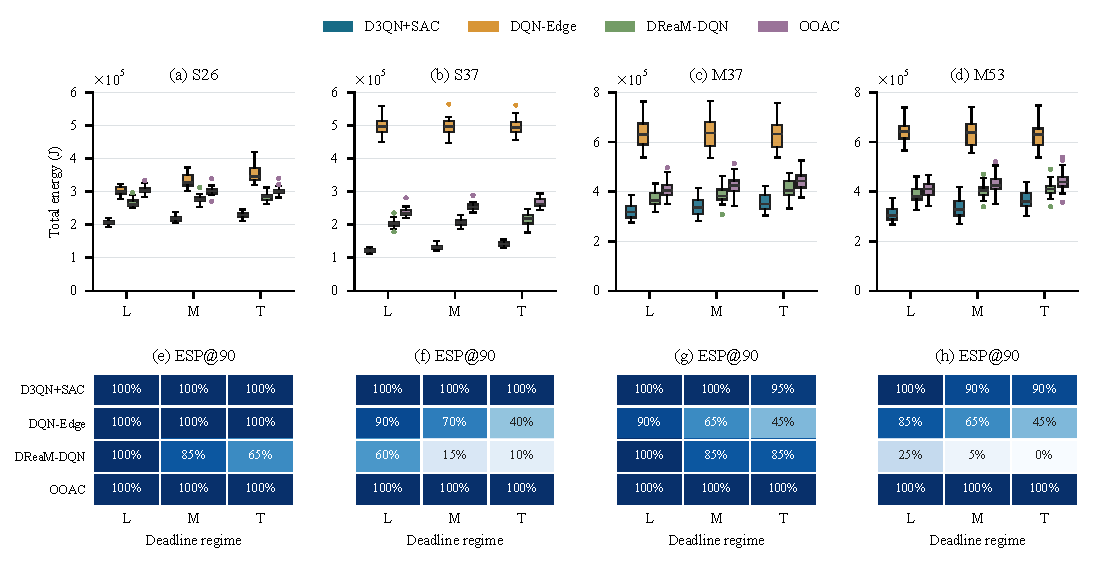
\includegraphics[width=\textwidth]{experiment_assets/main_comparison.pdf}
\caption{Main comparison on 20 matched, unseen workload seeds per
condition. Columns correspond to S26, S37, M37, and M53. In the upper
panels, boxes show the median and interquartile range of total active
computation energy; whiskers extend to the furthest observations within
1.5 interquartile ranges, and dots show observations outside the
whiskers. Lower panels report ESP@90. L, M, and T denote Loose, Medium,
and Tight deadline distributions. Reliability attainment is 100\% for
all methods. An empirical service-level feasible result requires
ESP@90 $\geq90\%$; low energy below this gate is not a feasible improvement.}
\label{fig:main_comparison}
\end{figure*}

\begin{table*}[t]
\centering
\caption{Total active computation energy (J): mean $\pm$ sample
standard deviation on the same 20 test seeds. Deadline feasibility is
reported in Fig.~\ref{fig:main_comparison}. Bold identifies the lowest
energy among empirically feasible methods in each condition.}
\label{tab:main_energy}
\footnotesize
\setlength{\tabcolsep}{7pt}
\renewcommand{\arraystretch}{1.08}
\begin{tabular}{@{}llrrr@{}}
\toprule
Scenario & Method & Loose & Medium & Tight \\
\midrule
S26 & D3QN+SAC & \textbf{206,301.27 $\pm$ 7,674.55} & \textbf{218,582.71 $\pm$ 9,004.38} & \textbf{229,668.81 $\pm$ 9,708.86} \\
 & DQN-Edge & 302,503.19 $\pm$ 12,679.50 & 333,163.60 $\pm$ 19,018.30 & 352,640.89 $\pm$ 24,430.03 \\
 & DReaM-DQN & 265,523.59 $\pm$ 12,543.93 & 277,161.73 $\pm$ 13,472.38 & 285,565.23 $\pm$ 12,765.79 \\
 & OOAC & 304,560.24 $\pm$ 12,500.09 & 302,308.85 $\pm$ 13,707.71 & 302,492.80 $\pm$ 12,803.92 \\
\midrule
S37 & D3QN+SAC & \textbf{121,572.94 $\pm$ 6,016.08} & \textbf{132,068.80 $\pm$ 7,423.62} & \textbf{142,052.08 $\pm$ 7,768.61} \\
 & DQN-Edge & 494,940.35 $\pm$ 26,979.60 & 496,496.87 $\pm$ 28,006.09 & 496,022.55 $\pm$ 29,002.06 \\
 & DReaM-DQN & 203,787.41 $\pm$ 13,267.21 & 206,969.85 $\pm$ 11,748.61 & 216,014.33 $\pm$ 19,493.04 \\
 & OOAC & 238,034.31 $\pm$ 14,159.96 & 254,903.74 $\pm$ 12,250.34 & 266,434.30 $\pm$ 13,773.49 \\
\midrule
M37 & D3QN+SAC & \textbf{320,956.10 $\pm$ 30,980.06} & \textbf{337,724.27 $\pm$ 34,575.94} & \textbf{357,541.30 $\pm$ 35,112.29} \\
 & DQN-Edge & 638,539.39 $\pm$ 58,726.93 & 638,592.71 $\pm$ 61,163.25 & 633,266.52 $\pm$ 60,541.28 \\
 & DReaM-DQN & 370,813.10 $\pm$ 32,388.93 & 389,029.88 $\pm$ 36,630.62 & 412,541.81 $\pm$ 38,516.52 \\
 & OOAC & 409,023.55 $\pm$ 37,223.79 & 426,940.73 $\pm$ 41,543.78 & 444,254.24 $\pm$ 40,864.44 \\
\midrule
M53 & D3QN+SAC & \textbf{309,983.80 $\pm$ 30,493.07} & \textbf{337,158.82 $\pm$ 39,198.63} & \textbf{366,341.92 $\pm$ 37,627.01} \\
 & DQN-Edge & 641,995.35 $\pm$ 49,112.30 & 637,580.02 $\pm$ 53,455.30 & 628,621.20 $\pm$ 54,312.97 \\
 & DReaM-DQN & 388,762.32 $\pm$ 33,748.03 & 403,988.49 $\pm$ 33,785.59 & 412,797.33 $\pm$ 33,307.17 \\
 & OOAC & 409,053.37 $\pm$ 35,906.93 & 430,066.42 $\pm$ 41,701.07 & 445,617.81 $\pm$ 44,094.60 \\

\bottomrule
\end{tabular}
\end{table*}

\subsubsection{Small Workflows}

In S26, the proposed method obtains ESP@90 $=100\%$ under all three
deadline distributions, with mean energy increasing from 206,301.27 J
under Loose deadlines to 229,668.81 J under Tight deadlines.
DQN-Edge and OOAC also attain 100\% ESP throughout S26, whereas
DReaM-DQN decreases from 100\% to 85\% and 65\% as deadlines become
less permissive. Relative to the lowest-energy feasible baseline in
each condition, the proposed method saves 22.30\%, 27.70\%, and
24.07\% for Loose, Medium, and Tight, respectively. The latter two
comparisons use OOAC, not the lower-energy but infeasible DReaM result.

In S37, the proposed method again attains 100\% ESP in every regime.
Its energy ranges from 121,572.94 to 142,052.08 J, yielding
46.68--48.93\% savings relative to OOAC, the lowest-energy feasible
baseline. DReaM-DQN has lower energy than OOAC but ESP of only
60\%, 15\%, and 10\%, and therefore cannot be ranked as a better
constrained solution. DQN-Edge meets the 90\% service gate only under
Loose deadlines. These results demonstrate the importance of
evaluating energy together with its service attainment, rather than
ranking policies by energy alone.

\subsubsection{Medium Workflows}

In M37, the proposed method reaches ESP of 100\%, 100\%, and 95\%
under Loose, Medium, and Tight deadlines, respectively. It reduces
energy by 13.45\% relative to feasible DReaM-DQN under Loose deadlines,
and by 20.90\% and 19.52\% relative to OOAC under Medium and Tight
deadlines. DReaM-DQN reaches only 85\% ESP in the latter two conditions.
OOAC reaches 100\% in all three, but with higher energy. The Tight
comparison is therefore a tradeoff within the feasible region, not
evidence that our policy has higher deadline ESP than OOAC.

For M53, the proposed method retains 100\% ESP under Loose deadlines
and attains 90\% under both Medium and Tight deadlines. Its respective
energy savings relative to OOAC are 24.22\%, 21.60\%, and 17.79\%.
These results meet the stated empirical 90\% service gate but not an
all-test-realizations-success requirement. OOAC remains more
conservative in deadline attainment, reaching 100\% ESP throughout.
DReaM-DQN and DQN-Edge do not meet the gate in any M53 condition.
Across all 12 conditions, our selected policies provide the lowest
energy among empirically feasible methods, with savings of
13.45--48.93\% against the lowest-energy feasible baseline.

\subsection{Resource Provision and Deadline-Distribution Robustness}
\label{subsec:resource_robustness}

The expanded resource configurations do not imply a monotonic change
in total active computation energy. For Small workflows, S37 consumes
38.15--41.07\% less energy than S26, depending on the deadline regime.
For Medium workflows, M53 consumes 3.42\% less energy than M37 under
Loose deadlines, almost the same energy under Medium deadlines, and
2.46\% more energy under Tight deadlines. More servers do not incur
an automatic idle-power charge in the adopted objective. Instead,
the measured difference depends on selected profiles, frequency
choices, contention, and the resulting execution durations.

Two additional aspects prevent interpreting these comparisons as a
pure hardware-capacity intervention. First, each configuration has
its own trained policy. Second, reference makespans and therefore
deadlines are recomputed on the respective server pools. The
results establish performance under each workload--resource
configuration, not the isolated causal effect of adding servers.

Within a configuration, however, the three deadline regimes use the
same checkpoint. Small-workflow policies preserve 100\% ESP while
their mean energy increases under tighter deadline distributions.
The Medium-workflow policies show a reduced margin: ESP reaches
95\% in M37-Tight and 90\% in M53-Medium/Tight. This contrast
supports robustness to deadline-distribution changes within the
evaluated scope, while showing that difficult unseen realizations
can still fail. It does not establish scale-independent transfer
of one policy between arbitrary workflow or server sizes.

\subsection{Ablation Study}
\label{subsec:ablation}

The ablations use S26 and test seeds 742000--742019, separate from
the main-comparison block. Each trained variant has one training run.
Table~\ref{tab:ablation} and Fig.~\ref{fig:ablation} report six variants.
\emph{Full} is the complete hierarchy. \emph{Full, $\rho=1$} evaluates
the same trained networks with frequency fixed at maximum; it is
an inference-time intervention, not a separately trained method.
\emph{High only, $\rho=1$} retrains the complete upper learner at
full frequency. \emph{HEFT+SAC} replaces learned placement by the
queue-aware HEFT-based dispatcher and retrains SAC under that dispatcher.
\emph{HEFT, $\rho=1$} is its non-learning full-frequency counterpart.
\emph{No deadline head} retrains the upper learner without its
deadline estimator, with frequency fixed at maximum. Reliability
attainment is 100\% in every ablation condition.

\begin{figure*}[t]
\centering
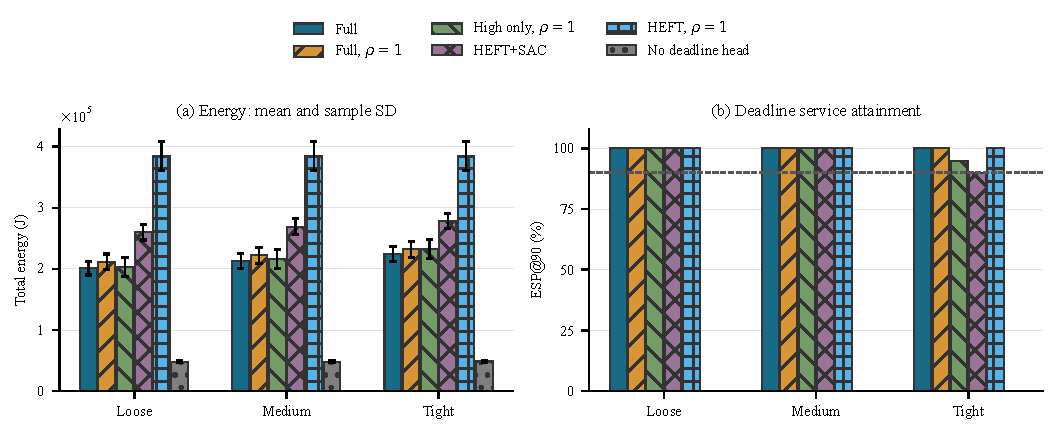
\includegraphics[width=\textwidth]{experiment_assets/ablation.pdf}
\caption{S26 structural ablations on 20 unseen test seeds.
Energy bars show the mean with sample-standard-deviation error bars;
the dashed line in the right panel marks the empirical ESP@90
service gate of 90\%. The very low energy of the no-deadline-head
variant is accompanied by zero ESP, so it is not a valid saving.
All results are conditional on one training run per trained variant.}
\label{fig:ablation}
\end{figure*}

\begin{table*}[t]
\centering
\caption{S26 ablations: energy (J), mean $\pm$ sample standard
deviation, and ESP@90 on 20 fixed test seeds. All reliability
attainment values are 100\%. Gray energy values fail the empirical
90\% ESP gate. Bold energy values are the lowest among feasible variants.}
\label{tab:ablation}
\scriptsize
\setlength{\tabcolsep}{4pt}
\renewcommand{\arraystretch}{1.12}
\begin{tabular}{@{}lrrrrrr@{}}
\toprule
& \multicolumn{2}{c}{Loose} & \multicolumn{2}{c}{Medium} & \multicolumn{2}{c}{Tight} \\
\cmidrule(lr){2-3}\cmidrule(lr){4-5}\cmidrule(l){6-7}
Variant & Energy (J) & ESP & Energy (J) & ESP & Energy (J) & ESP \\
\midrule
Full & \textbf{201,071.29 $\pm$ 11,024.15} & 100\% & \textbf{212,868.89 $\pm$ 12,545.21} & 100\% & \textbf{224,469.60 $\pm$ 12,838.52} & 100\% \\
Full, $\rho=1$ & 211,943.11 $\pm$ 12,478.92 & 100\% & 222,158.12 $\pm$ 13,499.18 & 100\% & 232,159.99 $\pm$ 13,122.15 & 100\% \\
High only, $\rho=1$ & 203,305.50 $\pm$ 15,853.78 & 100\% & 216,682.48 $\pm$ 15,727.77 & 100\% & 231,928.32 $\pm$ 15,565.62 & 95\% \\
HEFT+SAC & 260,141.52 $\pm$ 12,724.50 & 100\% & 269,414.45 $\pm$ 13,676.89 & 100\% & 278,090.85 $\pm$ 11,916.56 & 90\% \\
HEFT, $\rho=1$ & 384,508.56 $\pm$ 24,125.01 & 100\% & 384,508.56 $\pm$ 24,125.01 & 100\% & 384,508.56 $\pm$ 24,125.01 & 100\% \\
No deadline head & \textcolor{gray}{48,460.86 $\pm$ 1,806.66} & 0\% & \textcolor{gray}{48,458.77 $\pm$ 1,651.64} & 0\% & \textcolor{gray}{48,487.54 $\pm$ 1,662.90} & 0\% \\

\bottomrule
\end{tabular}
\end{table*}

\subsubsection{Contribution of Frequency Control}

Relative to evaluating Full at $\rho=1$, Full reduces mean energy
by 5.13\%, 4.18\%, and 3.31\% under Loose, Medium, and Tight
deadlines while retaining 100\% ESP. The benefit decreases as
deadlines become tighter, consistent with reduced room for slowing
execution. This intervention holds the learned network parameters
fixed, but not the complete placement trajectory: frequency changes
alter queues and can change later upper-level decisions. The measured
difference is therefore the net effect of frequency control under
the frozen policies, including its scheduling interactions.

\subsubsection{Contribution of Learned Placement}

Full consumes 22.71\%, 20.99\%, and 19.28\% less energy than
HEFT+SAC across the three regimes. Under Tight deadlines, HEFT+SAC
achieves 90\% ESP whereas Full achieves 100\%; both pass the stated
service gate, but with different robustness margins. HEFT+SAC itself
reduces energy by 27.68--32.34\% relative to HEFT at maximum frequency.
Thus, SAC can exploit slack under heuristic placement, but learned
placement is important to the lower energy of the complete system.
HEFT here is a reference heuristic, not a proved minimum-energy or
deadline-feasibility bound.

\subsubsection{Contribution of the Upper Deadline Estimator}

Removing the deadline head reduces mean energy to approximately
48,500 J but produces ESP $=0\%$ in all three regimes. The policy
therefore does not provide an admissible alternative to Full.
The full-frequency upper learner with its deadline head retained
achieves 100\%, 100\%, and 95\% ESP, providing a controlled contrast
with the no-head variant: both are independently trained at
full frequency. This comparison supports the necessity of
deadline-aware upper decisions in the tested system.
It does not individually identify the contribution of every queue,
critical-path, or credit-assignment term within that estimator.

Full also uses less energy than the independently trained upper-only
variant in every regime. Their Tight ESP values differ by one
successful test realization (20/20 versus 19/20). This observation
is consistent with a coordination benefit, but is not evidence of
training-seed-independent superiority of joint learning.

\subsection{Learning Dynamics}
\label{subsec:learning_dynamics}

Figure~\ref{fig:learning_dynamics} shows the recorded validation
energy and the minimum ESP across available validation blocks
during training. The curves use raw evaluation points without
smoothing and stop at the last saved evaluation; they are not
averages over repeated training runs. The Small configurations
reach high validation ESP earlier and fluctuate less afterward
than the Medium configurations. Low early energy coincides with
poor deadline attainment and should not be interpreted as a useful
energy optimum.

The Medium configurations continue to exhibit deadline fluctuations
after high-ESP checkpoints first appear. In particular, the last
M53 validation point is worse than some earlier points. Accordingly,
final testing uses a validation-selected checkpoint rather than the
last training episode. These curves demonstrate the importance of
constraint-aware checkpoint selection; they do not establish that
all four runs reached a stable optimization plateau.

\begin{figure*}[t]
\centering
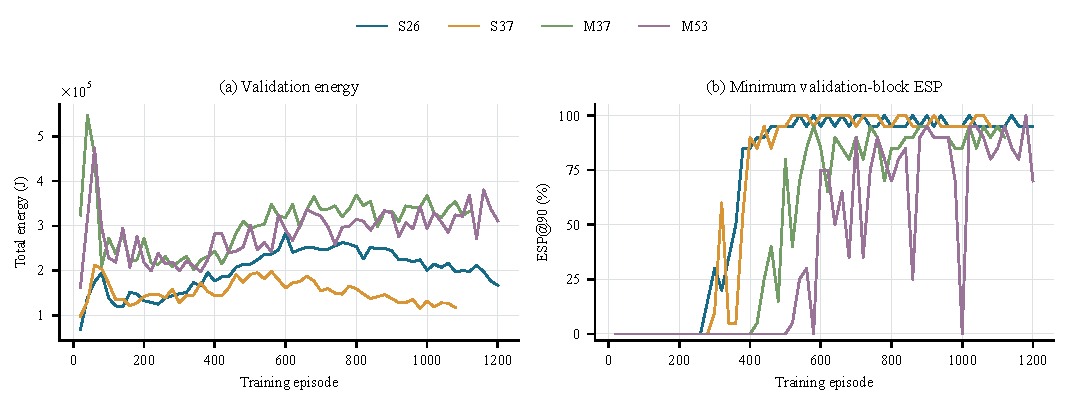
\includegraphics[width=\textwidth]{experiment_assets/learning_dynamics.pdf}
\caption{Recorded learning dynamics of the proposed method under
Medium deadlines. Energy is averaged over the available validation
blocks; deadline ESP is the minimum block value. Lines connect raw
evaluation points from one training run per configuration, without
smoothing or across-training-run confidence intervals. Curves stop
at the last saved evaluation, not necessarily the configured ceiling.}
\label{fig:learning_dynamics}
\end{figure*}

\subsection{Statistical Significance}
\label{subsec:significance}

We compare total energy using two-sided paired Wilcoxon signed-rank
tests. For each fixed test seed, relative energy reduction is
averaged equally over the four configurations and three deadline
regimes. This gives 20 seed-level contrasts, rather than treating
the 240 repeated condition-level observations as independent.
Table~\ref{tab:wilcoxon_energy} reports exact $p$-values and
corrections for the three baseline comparisons. All 20 aggregated
contrasts are positive for each baseline, which explains their
identical exact $p$-values. The comparisons remain significant
at level 0.05 after either correction.

These tests address energy differences across the evaluated
conditions, including conditions in which a baseline is infeasible.
They are not tests of deadline superiority or constrained optimality.
The inference is conditional on the selected policies and assumes
independent seed blocks and the signed-rank null's symmetry condition;
it does not quantify variability across independently trained policies.

\begin{table}[t]
\centering
\caption{Two-sided paired Wilcoxon signed-rank tests of total energy:
our method versus each baseline, using 20 seed-level contrasts.}
\label{tab:wilcoxon_energy}
\footnotesize
\setlength{\tabcolsep}{3.5pt}
\renewcommand{\arraystretch}{1.08}
\begin{tabular}{@{}lrrr@{}}
\toprule
Baseline & Raw $p$ & Bonferroni & BH--FDR \\
\midrule
DQN-Edge & $1.91\times10^{-6}$ & $5.72\times10^{-6}$ & $1.91\times10^{-6}$ \\
DReaM-DQN & $1.91\times10^{-6}$ & $5.72\times10^{-6}$ & $1.91\times10^{-6}$ \\
OOAC & $1.91\times10^{-6}$ & $5.72\times10^{-6}$ & $1.91\times10^{-6}$ \\
\bottomrule
\end{tabular}
\vspace{2pt}
\begin{minipage}{\columnwidth}
\footnotesize
Each contrast averages $(E_{\mathrm{baseline}}-E_{\mathrm{ours}})/
E_{\mathrm{baseline}}$ over 12 conditions for one seed. Both
corrections cover the three baseline comparisons. Energy significance
does not establish service-level feasibility.
\end{minipage}
\end{table}

\subsection{Scope and Limitations}
\label{subsec:experimental_limitations}

The four trained configurations demonstrate energy--service tradeoffs
on unseen workload realizations and different deadline distributions.
They do not demonstrate that one policy transfers unchanged across
all workflow sizes or server counts. Exploratory Medium-to-Large
transfer showed reduced deadline ESP, so uniform cross-scale
feasibility is not claimed. This limitation is distinct from the
within-configuration deadline-distribution tests in the main figure.

The current study also uses one training seed per reported trained
variant, historical differences in baseline checkpoint selection,
synthetically assigned workloads and data volumes, and a computation-only
energy objective. Reliability attainment is uniformly high under the
chosen fault rates, so these experiments do not establish a separate
energy or feasibility gain from reliability adaptation. Repeated
training, a fully uniform validation protocol, more demanding
reliability settings, and cross-scale deployment are needed before
making stronger reproducibility or generalization claims.


\bibliographystyle{IEEEtran}
\bibliography{references}

\end{document}
